\begin{samplecase}
{\bf Different level density models : n + ${}^{99}$Tc}\newline
To demonstrate the variety of level density models that we have added 
recently to TALYS, we include a sample case in which 3 different models 
are compared. The results are given in Fig. \ref{tccum} for
the cumulative number of discrete levels and in Fig.\ref{tcnp} for the (n,p)
cross section.
\subsubsection{Case a: Constant Temperature Model}
The input file is

\VerbatimInput{\samples n-Tc099-ld1/org/talys.inp}

This is the default calculation: TALYS use the local CTM level density for
its calculations
\subsubsection{Case b: Back-shifted Fermi gas Model}
The input file is

\VerbatimInput{\samples n-Tc099-ld2/org/talys.inp}

\subsubsection{Case c: Hartree-Fock Model}
The input file is

\VerbatimInput{\samples n-Tc099-ld5/org/talys.inp}

The level density files contain a lot of metadata. For example, {\em ld043100.tot} looks as follows
{\small \begin{verbatim}

# header:
#   title: Tc100 level density
#   source: TALYS-2.0
#   user: Arjan Koning
#   date: 2023-12-14
#   format: YANDF-0.1
# residual:
#   Z: 43
#   A: 100
#   nuclide: Tc100
# parameters:
#   ldmodel keyword: 1
#   level density model: Gilbert-Cameron
#   Collective enhacement: n
#   a(Sn) [MeV^-1]:  1.616190E+01
#   asymptotic a [MeV^-1]:  1.336739E+01
#   shell correction [MeV]:  3.021460E+00
#   damping gamma:  9.330641E-02
#   pairing energy [MeV]:  0.000000E+00
#   adjusted pairing shift [MeV]:  0.000000E+00
#   separation energy [MeV]:  6.764404E+00
#   discrete spin cutoff parameter:  8.238095E+00
#   spin cutoff parameter(Sn):  2.342199E+01
#   matching energy [MeV]:  4.445303E+00
#   temperature [MeV]:  6.575356E-01
#   E0 [MeV]: -2.006161E+00
#   Nlow: 8
#   Ntop: 17
#   ctable:  1.000000E-20
#   ptable:  1.000000E-20
# observables:
#   experimental D0 [eV]:  1.200000E+01
#   experimental D0 unc. [eV]:  1.300000E+00
#   theoretical D0 [eV]:  1.200798E+01
#   Chi-2 D0:  3.767498E-05
#   C/E D0:  1.000665E+00
#   Frms D0:  1.000003E+00
#   Erms D0:  1.000003E+00
#   Chi-2 per level:  4.622709E-02
#   Frms per level:  1.016615E+00
#   Erms per level:  1.000363E+00
#   average deviation per level:  5.333306E-02
# datablock:
#   quantity: level density
#   columns: 6
#   entries: 79
##       E            Level      N_cumulative     Total LD           a      
##     [MeV]           []             []          [MeV^-1]       [MeV^-1]  
   3.194900E-01     9            9.020750E+00   5.225714E+01   1.708033E+01
   3.351600E-01    10            9.849436E+00   5.351747E+01   1.707764E+01
   3.409800E-01    11            1.016229E+01   5.399327E+01   1.707664E+01
   3.555800E-01    12            1.095939E+01   5.520555E+01   1.707412E+01
   4.006300E-01    13            1.353307E+01   5.912044E+01   1.706639E+01
   4.243600E-01    14            1.496155E+01   6.129303E+01   1.706232E+01
   4.403800E-01    15            1.595550E+01   6.280470E+01   1.705957E+01
   4.542000E-01    16            1.683263E+01   6.413869E+01   1.705721E+01
   4.567900E-01    17            1.699907E+01   6.439182E+01   1.705677E+01
   4.580900E-01    18            1.708286E+01   6.451926E+01   1.705655E+01
...................
\end{verbatim} } \renewcommand{\baselinestretch}{1.07}\small\normalsize
\noindent

\end{samplecase}
\begin{figure}
\centering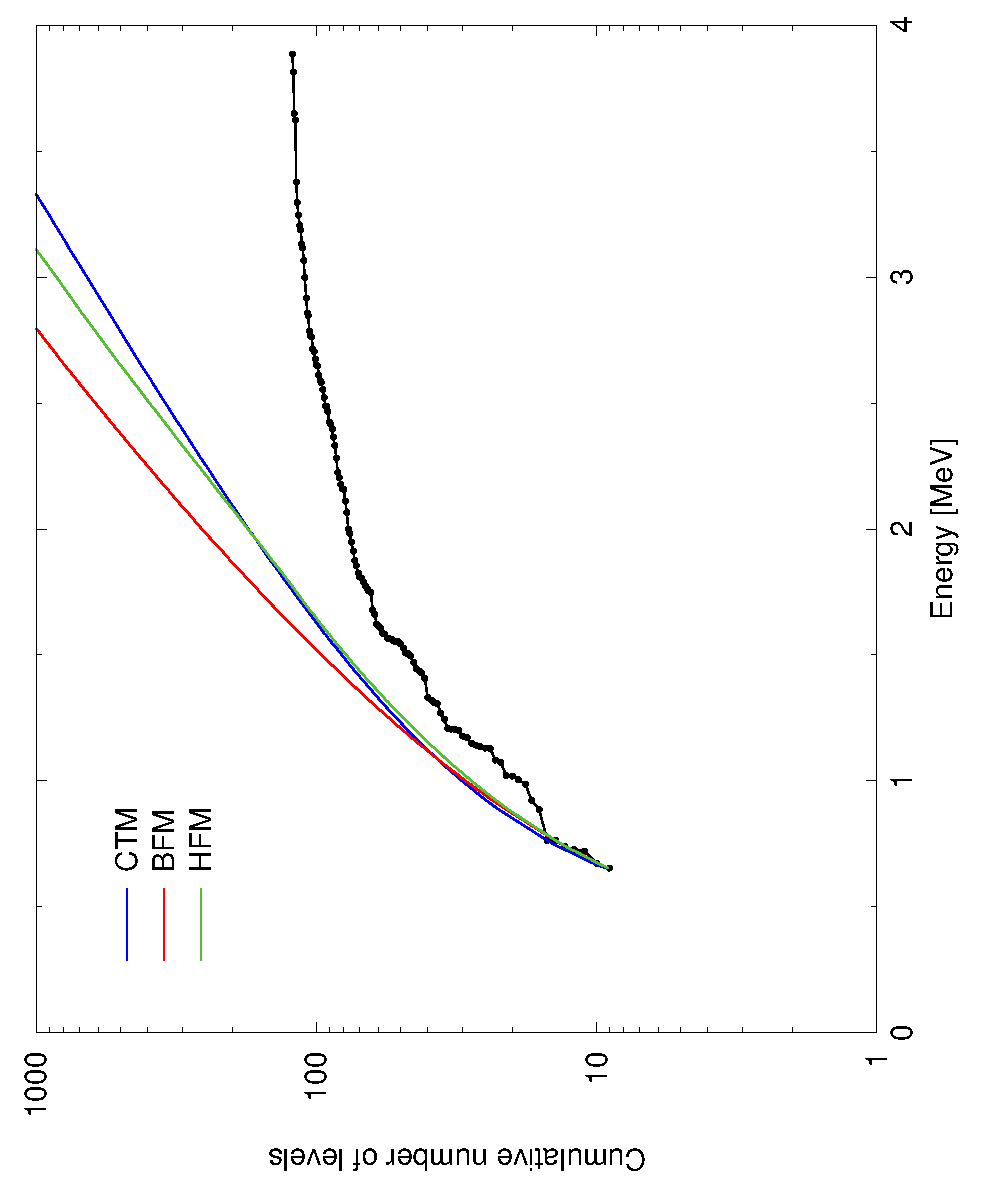
\includegraphics[scale=0.5,angle=270]{ldc}
\caption{Cumulative number of discrete levels of $^{99}$Tc for different 
level density models.}
\label{tccum}
\end{figure}
\begin{figure}
\centering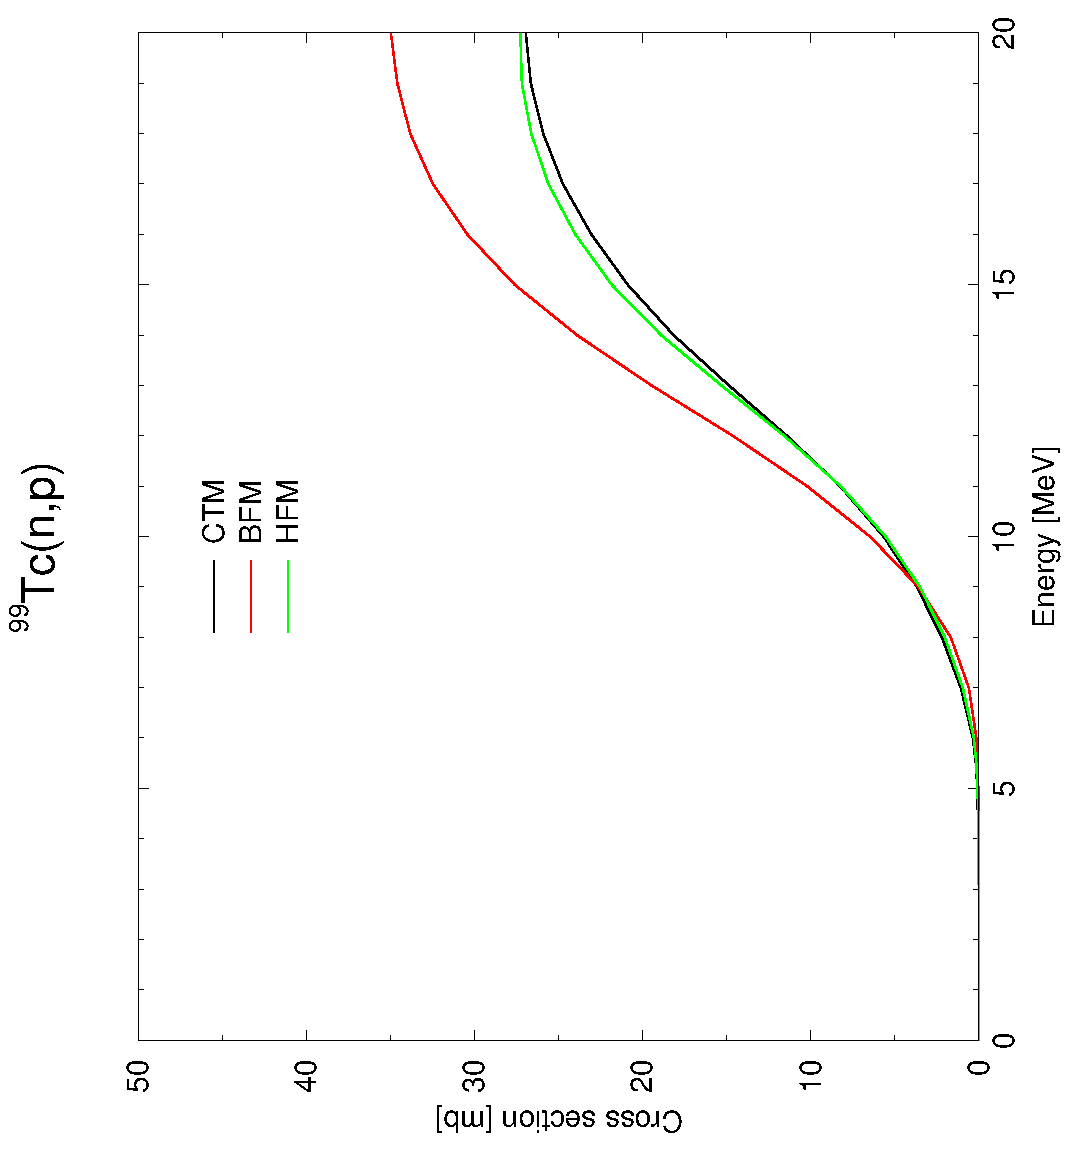
\includegraphics[scale=0.5,angle=270]{rp042099}
\caption{$^{99}$Tc(n,p) cross section for different 
level density models.}
\label{tcnp}
\end{figure}
